\documentclass[11pt]{article}
\usepackage[T1]{fontenc}
\usepackage[utf8]{inputenc}
\usepackage[dvipsnames]{xcolor}
\usepackage{amsmath,amsthm}
\usepackage{newtxtext,newtxmath}
\usepackage[margin=1in,headheight=15pt]{geometry}
\usepackage{microtype,mathtools,booktabs,array,graphicx}
\usepackage{enumitem,fancyhdr,listings,tcolorbox}
\usepackage[colorlinks=true,linkcolor=MidnightBlue,citecolor=MidnightBlue,urlcolor=MidnightBlue]{hyperref}
\usepackage[nameinlink,noabbrev]{cleveref}
\usepackage{bookmark}
\definecolor{ink}{HTML}{19354B}
\definecolor{lightink}{HTML}{F1F5F8}
\hypersetup{pdftitle={Exact Records in the Square-Root-of-Three Walk},pdfauthor={Research report prepared with ChatGPT},pdfsubject={A conjectured record recurrence, exact first passages, and an even-trace extension}}
\pagestyle{fancy}
\fancyhf{}
\fancyhead[L]{\small\textsc{Exact records in a quadratic walk}}
\fancyhead[R]{\small September 2026}
\fancyfoot[C]{\thepage}
\renewcommand{\headrulewidth}{0.3pt}
\setlength{\parskip}{4pt}
\setlength{\parindent}{1.2em}
\setlength{\emergencystretch}{2em}
\newtheorem{theorem}{Theorem}[section]
\newtheorem{lemma}[theorem]{Lemma}
\newtheorem{proposition}[theorem]{Proposition}
\newtheorem{corollary}[theorem]{Corollary}
\theoremstyle{definition}
\newtheorem{definition}[theorem]{Definition}
\newtheorem{remark}[theorem]{Remark}
\numberwithin{equation}{section}
\newcommand{\fl}[1]{\left\lfloor #1\right\rfloor}
\newcommand{\ce}[1]{\left\lceil #1\right\rceil}
\newcommand{\fr}[1]{\left\{#1\right\}}
\newcommand{\NN}{\mathbb N}
\newcommand{\ZZ}{\mathbb Z}
\newcommand{\odd}{\varepsilon}
\newcommand{\isqrt}{\operatorname{isqrt}}
\newcommand{\Rs}{\mathcal R}
\lstset{basicstyle=\ttfamily\small,columns=fullflexible,keepspaces=true,breaklines=true,frame=single,rulecolor=\color{black!20},showstringspaces=false,aboveskip=10pt,belowskip=10pt}
\setlist{nosep,leftmargin=1.5em}
\begin{document}
\hypersetup{pageanchor=false}
\begin{titlepage}
\vspace*{0.45in}
{\color{ink}\Large\scshape Discrete mathematics and integer sequences\par}
\vspace{0.4in}
{\color{ink}\huge\bfseries Exact Records in the\par Square-Root-of-Three Walk\par}
\vspace{0.25in}
{\Large A proof of the Arias de Reyna--van de Lune recurrence\par and an even-trace extension\par}
\vspace{0.35in}
{\large Research report prepared with ChatGPT\par}
{\large September 19, 2026\par}
\vspace{0.4in}
\begin{abstract}
Consider the integer-valued walk
\[
 S(N)=\sum_{n=1}^{N}(-1)^{\lfloor n\sqrt3\rfloor},\qquad S(0)=0.
\]
A conjecture, reproduced in the recent work of Bruin and Fokkink, gives a four-phase linear recurrence for the first occurrences of new values of this walk. We prove that recurrence by identifying an exact first-passage lift
\[
 F(m)=4\lfloor(2+\sqrt3)m\rfloor-m+7.
\]
The successive record positions are exactly $R_{4q+j}=F^q(j)$ for $0\le j\le3$. The proof establishes minimality of every first passage, not merely the value at a proposed record. We obtain the rational generating function of the full record sequence, explicit closed forms, and the sharp asymmetry
\[
 \limsup_{N\to\infty}\frac{S(N)}{\log N}
 =\frac1{2\log(2+\sqrt3)},\qquad
 \liminf_{N\to\infty}\frac{S(N)}{\log N}
 =-\frac3{2\log(2+\sqrt3)}.
\]
An extension treats every even integer $D\ge4$ and the quadratic slope $(D+\sqrt{D^2-4})/2$. All proofs are elementary and independent of the supplied exact-integer computations.
\end{abstract}
\vfill
\begin{tcolorbox}[colback=lightink,colframe=ink,boxrule=0.5pt]
\small\textbf{Status and scope.} The selected conjecture is explicitly described as experimental in \cite[Section~2, p.~7]{BF}, consulted on September 19, 2026. This report supplies a complete proof of that specific recurrence and the extension stated here. It does not solve the general conjecture for every quadratic irrational. The argument has been checked computationally but has not been independently refereed or formally verified; historical priority beyond the sources inspected is not certified.
\end{tcolorbox}
\end{titlepage}
\hypersetup{pageanchor=true}
\tableofcontents
\newpage

\section{The problem and the main result}\label{sec:problem}
The walk in this report has no random choices. Its increments are determined by the parity of $\lfloor n\sqrt3\rfloor$. Starting from $0$, its first values are
\[
0,-1,-2,-3,-2,-1,0,1,0,-1,-2,-3,\ldots.
\]
A positive integer $N$ is a \emph{record position} if $S(N)$ has not occurred at any earlier position, including position $0$. Because every step is $+1$ or $-1$, these positions are precisely the first passages to new positive maxima or new negative minima. We include $R_0=0$ as an initial record and list all subsequent records increasingly.

Arias de Reyna and van de Lune studied such oscillating sums in \cite{ARL}. Bruin and Fokkink reproduce the following conjectured recurrence, correcting a typographical error in its first line \cite[Section~2, p.~7]{BF}:
\begin{align}
 R_{4q+1}&=2R_{4q}+R_{4q-1}+1,\label{eq:conj1}\\
 R_{4q+2}&=R_{4q+1}+2R_{4q}+1,\label{eq:conj2}\\
 R_{4q+3}&=R_{4q+2}+2R_{4q}+1,\label{eq:conj3}\\
 R_{4q+4}&=2R_{4q+3}+R_{4q}+1.\label{eq:conj4}
\end{align}
Here $q\ge0$, $R_0=0$, and $R_{-1}=0$ is only a boundary convention. The mathematical question is whether this recurrence generates \emph{all and only} the actual records.

Set
\begin{equation}\label{eq:constants}
 \beta=2-\sqrt3,\quad \gamma=2+\sqrt3=\beta^{-1},\quad
 \mu=\gamma^2=7+4\sqrt3,
\end{equation}
and define
\begin{equation}\label{eq:BFdef}
 B(m)=\lfloor\gamma m\rfloor,\qquad
 F(m)=4B(m)-m+7\qquad(m\ge0).
\end{equation}
The notation $F^q$ means $q$-fold composition, with $F^0(m)=m$; it is not an ordinary power.

\begin{theorem}[Complete record theorem]\label{thm:main}
For every $q\ge0$ and $0\le j\le3$, the record positions and their values are
\begin{equation}\label{eq:main}
 R_{4q+j}=F^q(j),\qquad
 S(R_{4q+j})=
 \begin{cases}q,&j=0,\\-(3q+j),&1\le j\le3.\end{cases}
\end{equation}
These positions are strictly increasing in their displayed order and exhaust the records. They satisfy \eqref{eq:conj1}--\eqref{eq:conj4}; thus the stated conjecture is true.
\end{theorem}

The first few blocks make the asymmetric pattern visible.
\begin{center}
\begin{tabular}{r|rrrr|c}
\toprule
$q$ & $R_{4q}$ & $R_{4q+1}$ & $R_{4q+2}$ & $R_{4q+3}$ & Values in the block\\
\midrule
0&0&1&2&3&$0,-1,-2,-3$\\
1&7&18&33&48&$1,-4,-5,-6$\\
2&104&257&466&675&$2,-7,-8,-9$\\
3&1455&3586&6497&9408&$3,-10,-11,-12$\\
4&20272&49953&90498&131043&$4,-13,-14,-15$\\
5&282359&695762&1260481&1825200&$5,-16,-17,-18$\\
\bottomrule
\end{tabular}
\end{center}
The proof has two logically separate parts. First, a decomposition into constant-sign runs determines the true first-passage map. Second, a two-dimensional affine identity turns its iterates into linear recurrences. This separation prevents a common experimental pitfall: checking that a proposed position attains a large value does not establish that it is the \emph{first} position to do so.

\begin{figure}[htbp]
\centering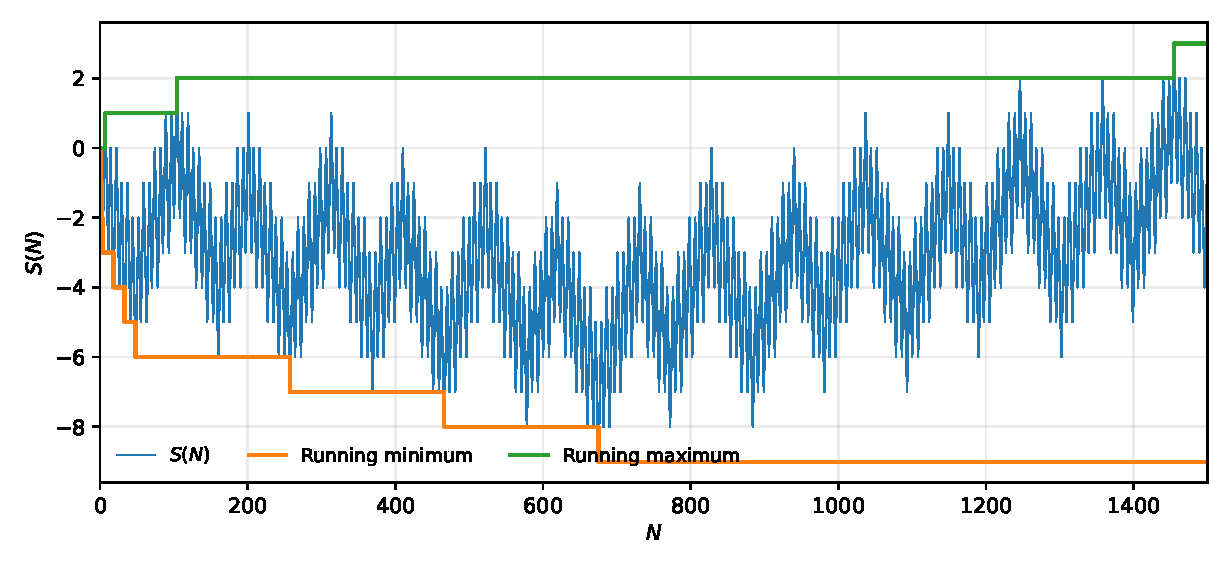
\includegraphics[width=\linewidth]{figures/walk_and_records.pdf}
\caption{The walk and its exact running extrema through $N=1500$. The three-to-one imbalance in new negative and positive record levels is a theorem, not an inference from the plot.}
\label{fig:walk}
\end{figure}

\section{Constant-sign runs and a shrinking identity}\label{sec:runs}
\subsection{Why the run endpoints are Beatty numbers}
Since $\sqrt3=2-\beta$ and $\beta n$ is irrational for $n\ge1$,
\begin{equation}\label{eq:sign}
 (-1)^{\lfloor n\sqrt3\rfloor}
 =(-1)^{2n-\lceil\beta n\rceil}
 =-(-1)^{\lfloor\beta n\rfloor}.
\end{equation}
Thus the sign is constant while $\lfloor\beta n\rfloor$ is constant. More precisely, for every $k\ge1$,
\begin{equation}\label{eq:run}
 B(k-1)<n\le B(k)
 \quad\Longrightarrow\quad
 \lfloor\beta n\rfloor=k-1,
 \qquad S(n)-S(n-1)=(-1)^k.
\end{equation}
To check the endpoints, multiply $k-1<\beta n<k$ by $\gamma$. The resulting inequalities are equivalent to
$\lfloor\gamma(k-1)\rfloor<n\le\lfloor\gamma k\rfloor$.
No endpoint ambiguity is possible because $\gamma k$ is nonintegral for $k>0$.

Let
\[
 T(k)=\lfloor\beta k\rfloor,\qquad T(0)=0.
\]
The relation $\gamma=4-\beta$ gives, for $k\ge1$,
\begin{equation}\label{eq:BfromT}
 B(k)=4k-T(k)-1.
\end{equation}
The first run has length $3$. Every later run has length $3$ or $4$, since
\begin{equation}\label{eq:lengths}
 B(k)-B(k-1)=4-\bigl(T(k)-T(k-1)\bigr)\quad(k\ge2).
\end{equation}
The short later runs occur at very specific run numbers: $T(k)$ increases at $k$ exactly when
\begin{equation}\label{eq:short}
 k=\lceil\gamma\ell\rceil=B(\ell)+1
 \quad\text{for some integer }\ell\ge1.
\end{equation}
Indeed, the event is $\beta(k-1)<\ell<\beta k$, with the harmless weak/strict endpoint conventions again equivalent by irrationality.

\begin{lemma}[Endpoint renormalization]\label[lemma]{lem:endpoint}
For every integer $k\ge1$,
\begin{equation}\label{eq:endpoint}
 \boxed{\quad S(B(k))=S(T(k))+1-4\odd(k),\quad}
\end{equation}
where $\odd(k)=k\bmod2$ belongs to $\{0,1\}$.
\end{lemma}
\begin{proof}
If all runs had length four, their signed total through run $k$ would be
$4\sum_{i=1}^k(-1)^i=-4\odd(k)$. Shortening the first, negative run by one contributes $+1$.
Each remaining short run has index $i=B(\ell)+1$ by \eqref{eq:short}; shortening that run changes the total by
\[
 -(-1)^i=(-1)^{B(\ell)}.
\]
There are exactly $T(k)$ such later short runs through run $k$. Finally,
$B(\ell)=2\ell+\lfloor\sqrt3\ell\rfloor$, so their total correction is
\[
 \sum_{\ell=1}^{T(k)}(-1)^{B(\ell)}=S(T(k)).
\]
Adding the three contributions proves the identity, including $k=1$.
\end{proof}

The addition in \eqref{eq:endpoint} is $-3$ at the end of a negative run and $+1$ at the end of a positive run. This is the exact origin of the three negative records for every positive record.

\subsection{An exact formula at every integer}
For $N\ge1$, put
\begin{equation}\label{eq:fullparameters}
 k=T(N)+1,\qquad m=T(k),\qquad d=B(k)-N.
\end{equation}
The integer $N$ lies in run $k$. Moving from $N$ to its endpoint adds $(-1)^k d$. Consequently,
\begin{equation}\label{eq:full}
 \boxed{S(N)=S(m)+1-4\odd(k)-(-1)^k d.}
\end{equation}
Together with $S(0)=0$, this determines every value exactly. The new argument satisfies
\[
 0\le m\le\beta^2N+\beta<N/2\qquad(N\ge1),
\]
because $\beta<1/3$ and $\beta^2+\beta<1/2$. In particular the recursion terminates after $O(\log(N+1))$ steps.

\begin{remark}[A base case that matters]
Equation \eqref{eq:BfromT} is valid only for $k\ge1$. At $k=0$, both $B(0)$ and $T(0)$ are zero, and there is no $-1$. The code treats zero separately rather than extending the positive-argument floor identity beyond its domain.
\end{remark}

\section{First passages: proof of minimality}\label{sec:first}
For $h\ge1$, let $L_h$ be the first position where $S=-h$, and let $U_h$ be the first position where $S=h$, when these positions exist. Put $U_0=0$. The following theorem also establishes that all these first passages exist.

\begin{lemma}[A useful pair of run numbers]\label[lemma]{lem:fiber}
For $m\ge0$,
\begin{equation}\label{eq:fiber}
 T(B(m)+2)=m.
\end{equation}
For $m\ge1$, the first run number $k$ with $T(k)\ge m$ is $B(m)+1$.
\end{lemma}
\begin{proof}
Write $u=\{\gamma m\}$, allowing $u=0$ when $m=0$. Then
\[
 \beta(B(m)+2)=m+\beta(2-u).
\]
The final summand lies strictly between $0$ and $1$, since $0\le u<1$ and $2\beta<1$. This proves \eqref{eq:fiber}.
For positive $m$, the inequality $\lfloor\beta k\rfloor\ge m$ is equivalent to $k\ge\lceil\gamma m\rceil=B(m)+1$.
\end{proof}

\begin{theorem}[First-passage lift]\label{thm:first}
Define temporarily $\widetilde F(m)=B(B(m)+2)$. Then
\begin{align}
 U_{h+1}&=\widetilde F(U_h) &&(h\ge0),\label{eq:Ufirst}\\
 L_1&=1,\quad L_2=2,\quad L_3=3,\qquad
 L_{h+3}=\widetilde F(L_h) &&(h\ge1).\label{eq:Lfirst}
\end{align}
\end{theorem}
\begin{proof}
The first run consists of three negative steps, proving the three initial negative first passages.

Consider a positive target $h+1$. A first passage to that target must occur during a positive run, whose index $k$ is even. By \cref{lem:endpoint}, the endpoint of this run reaches the target if and only if
\[
 S(T(k))+1\ge h+1,\quad\text{or equivalently }S(T(k))\ge h.
\]
Assume inductively that $U_h$ is known, with $U_0=0$. The smallest possible argument of $S$ satisfying this inequality is $m=U_h$. For $h>0$, the step at $m$ is positive, so $B(m)$ is even. This is also true at $m=0$. For $m>0$ the first eligible run number before imposing parity is $B(m)+1$, which is odd. The first eligible \emph{even} run is therefore
\[
 k_0=B(m)+2.
\]
When $m=0$, the first positive run is $k_0=2$, which is the same formula. By \cref{lem:fiber}, $T(k_0)=m$. Its endpoint has value exactly $h+1$, not a larger value. As this run is increasing, its first occurrence of $h+1$ is its endpoint $B(k_0)$. Every earlier positive run has endpoint below the target. This proves \eqref{eq:Ufirst}, including its first-passage assertion.

For a negative target $-(h+3)$ with $h\ge1$, a first passage must occur during an odd run. Its endpoint reaches the target exactly when
\[
 S(T(k))-3\le-(h+3),\quad\text{or equivalently }S(T(k))\le-h.
\]
The smallest eligible argument is $m=L_h$. The step at $m$ is negative, so $B(m)$ is odd. Hence $B(m)+1$ is even, and the first eligible odd run is again $k_0=B(m)+2$. Its reduced argument is exactly $m$, and its endpoint has value exactly $-(h+3)$. No earlier negative run reaches the target. The run is decreasing, so the endpoint is its first occurrence. This proves \eqref{eq:Lfirst}.

Starting from $U_0$ and $L_1,L_2,L_3$, these constructions inductively produce every positive and negative level, establishing existence as well as minimality.
\end{proof}

\section{The arithmetic of the lift}\label{sec:lift}
\begin{lemma}[Two affine identities]\label[lemma]{lem:affine}
For every $m\ge0$,
\begin{align}
 B(B(m)+2)&=4B(m)-m+7=F(m),\label{eq:liftidentity}\\
 B(F(m))&=15B(m)-4m+26.\label{eq:secondlift}
\end{align}
\end{lemma}
\begin{proof}
Write $u=\{\gamma m\}$ and use $\gamma^2=4\gamma-1$. Then
\[
 \gamma B(m)=4B(m)-m+\beta u.
\]
It follows that
\[
 B(B(m)+2)=4B(m)-m+\lfloor2\gamma+\beta u\rfloor.
\]
The expression inside the last floor lies in $[2\gamma,2\gamma+\beta)$, which is contained in $(7,8)$. This proves the first identity.
Applying $\gamma$ to $F(m)$ gives
\[
 \gamma F(m)=15B(m)-4m+7\gamma+\beta^2u.
\]
Here $4\beta-1=\beta^2$ has been used. Since
\[
 26<7\gamma\le7\gamma+\beta^2u<7\gamma+\beta^2<27,
\]
the second identity follows. The same computation works at $m=0$.
\end{proof}

\subsection{Exhausting the ordered record sequence}
By \cref{thm:first,lem:affine},
\begin{equation}\label{eq:closedfirst}
 U_q=F^q(0),\qquad L_{3q+j}=F^q(j)\quad(1\le j\le3).
\end{equation}
The map $F$ is strictly increasing on the nonnegative integers: $B(m+1)-B(m)\ge3$ implies $F(m+1)-F(m)\ge11$. Also $F(0)=7>3$. Therefore
\[
 F^q(0)<F^q(1)<F^q(2)<F^q(3)<F^{q+1}(0).
\]
Every record is a first passage to a positive or negative integer, and all such first passages occur in \eqref{eq:closedfirst}. This proves \eqref{eq:main}, its ordering, and its exhaustiveness.

\subsection{A constant-coefficient recurrence}
For a fixed seed $s\ge0$, write $x_q=F^q(s)$ and $y_q=B(x_q)$. The affine identities give
\begin{equation}\label{eq:matrix}
 \begin{pmatrix}x_{q+1}\\y_{q+1}\end{pmatrix}
 =A\begin{pmatrix}x_q\\y_q\end{pmatrix}+b,
 \qquad
 A=\begin{pmatrix}-1&4\\-4&15\end{pmatrix},\quad
 b=\begin{pmatrix}7\\26\end{pmatrix}.
\end{equation}
The matrix has trace $14$ and determinant $1$, so $A^2-14A+I=0$. For an affine recurrence $v_{q+1}=Av_q+b$, this yields
\[
 v_{q+2}-14v_{q+1}+v_q=Ab-13b.
\]
The first component on the right is $6$. We have proved:
\begin{proposition}\label[proposition]{prop:scalar}
Every orbit of $F$ satisfies
\begin{equation}\label{eq:scalar}
 x_{q+2}=14x_{q+1}-x_q+6.
\end{equation}
In particular, the full record sequence satisfies
\begin{equation}\label{eq:fullrec}
 R_{n+8}=14R_{n+4}-R_n+6\qquad(n\ge0).
\end{equation}
\end{proposition}

\section{Recovering the conjectured four-phase recurrence}\label{sec:original}
To avoid confusing the run endpoints $B(m)$ with a block label, put
\[
 A_q=F^q(0),\quad C_q=F^q(1),\quad E_q=F^q(2),\quad H_q=F^q(3).
\]
All four sequences satisfy \eqref{eq:scalar}. We claim
\begin{align}
 C_{q+1}-2A_{q+1}-H_q&=1,\label{eq:res1}\\
 E_q-C_q-2A_q&=1,\label{eq:res2}\\
 H_q-E_q-2A_q&=1,\label{eq:res3}\\
 A_{q+1}-2H_q-A_q&=1.\label{eq:res4}
\end{align}
Each left-hand side, as a sequence $Z_q$, satisfies
\[
 Z_{q+2}=14Z_{q+1}-Z_q-12,
\]
because its coefficients add to $-2$. The initial values
\[
\begin{array}{c|rrrr}
q&A_q&C_q&E_q&H_q\\\hline
0&0&1&2&3\\
1&7&18&33&48\\
2&104&257&466&675
\end{array}
\]
show $Z_0=Z_1=1$ in each case. The constant sequence $1$ satisfies the same recurrence, proving all four identities by induction.

The first identity gives \eqref{eq:conj1} for $q\ge1$ after shifting the block index. Its $q=0$ case is $R_1=1$ with $R_0=R_{-1}=0$. The remaining three identities are exactly \eqref{eq:conj2}--\eqref{eq:conj4}. This completes the proof of \cref{thm:main} in the precise form in which the conjecture was stated.

\section{Generating functions and closed forms}\label{sec:gf}
\subsection{A rational generating function for all records}
Let $\mathscr R(z)=\sum_{n\ge0}R_nz^n$, as a formal power series. Multiplying \eqref{eq:fullrec} by powers of $z$ and inserting the first eight values yields
\[
 (1-14z^4+z^8)\mathscr R(z)
 =z+2z^2+3z^3+7z^4+4z^5+5z^6+6z^7+\frac{6z^8}{1-z}.
\]
Consequently,
\begin{equation}\label{eq:gf}
 \boxed{\mathscr R(z)=
 \frac{z+z^2+z^3+4z^4-3z^5+z^6+z^7}
 {(1-z)(1-14z^4+z^8)}.}
\end{equation}
Thus an integer sequence originally defined through infinitely many irrational floor comparisons has a rational generating function when restricted to its record positions.

For the four separate phases, let $G_s(z)=\sum_{q\ge0}F^q(s)z^q$. With $H(z)=(1-z)(1-14z+z^2)$, the numerators are
\begin{center}
\begin{tabular}{c|c|c}
\toprule
$s$ & Initial orbit values & $G_s(z)$\\
\midrule
0&$0,7,104,1455,\ldots$&$z(7-z)/H(z)$\\
1&$1,18,257,3586,\ldots$&$(1+3z+2z^2)/H(z)$\\
2&$2,33,466,6497,\ldots$&$(2+3z+z^2)/H(z)$\\
3&$3,48,675,9408,\ldots$&$(3+3z)/H(z)$\\
\bottomrule
\end{tabular}
\end{center}
These formulas follow directly by multiplying \eqref{eq:scalar} by $z^{q+2}$ and summing. Equivalently,
$\mathscr R(z)=\sum_{s=0}^3z^sG_s(z^4)$.

\subsection{Closed forms without nested floors}
The shift $x_q+\tfrac12$ removes the constant in \eqref{eq:scalar}. Its characteristic roots are $\mu$ and $\mu^{-1}$. Therefore
\begin{equation}\label{eq:closed}
 \boxed{R_{4q+s}=c_s\mu^q+d_s\mu^{-q}-\frac12,\qquad0\le s\le3,}
\end{equation}
where
\begin{center}
\begin{tabular}{c|cc}
\toprule
$s$&$c_s$&$d_s$\\
\midrule
0&$\frac14+\frac1{2\sqrt3}$&$\frac14-\frac1{2\sqrt3}$\\[3pt]
1&$\frac34+\frac1{\sqrt3}$&$\frac34-\frac1{\sqrt3}$\\[3pt]
2&$\frac54+\frac2{\sqrt3}$&$\frac54-\frac2{\sqrt3}$\\[3pt]
3&$\frac74+\frac3{\sqrt3}$&$\frac74-\frac3{\sqrt3}$\\
\bottomrule
\end{tabular}
\end{center}
To verify the table, its entries give $x_0=s$ and $x_1=F(s)$, and each expression satisfies \eqref{eq:scalar}; uniqueness then proves \eqref{eq:closed}. The irrational quantities cancel to integers exactly. For computation, the integer recurrence is preferable to numerical evaluation of this closed form.

\section{Exact extrema and sharp asymptotic behavior}\label{sec:asymptotics}
\subsection{An exact prefix theorem}
\begin{corollary}\label[corollary]{cor:envelopes}
For the unique $q\ge0$ and $0\le j\le3$ such that
\[
 R_{4q+j}\le N<R_{4q+j+1},
\]
one has
\begin{equation}\label{eq:exactextrema}
 \min_{0\le n\le N}S(n)=-(3q+j),\qquad
 \max_{0\le n\le N}S(n)=q.
\end{equation}
\end{corollary}
\begin{proof}
At $R_{4q}$ the positive record is $q$, and the preceding negative records have already reached $-3q$. Each of the next three records decreases the minimum by one, and none changes the maximum. The next positive record occurs only at $R_{4q+4}$. Exhaustiveness in \cref{thm:main} rules out any other change between the listed positions. The initial block $q=0$ obeys the same convention.
\end{proof}

\subsection{The logarithmic constants}
All $c_s$ in \eqref{eq:closed} are positive. Since there are only four phases,
\begin{equation}\label{eq:recordlogs}
 \log R_{4q+s}=q\log\mu+O(1)\qquad(q\to\infty),
\end{equation}
uniformly for $s=0,1,2,3$. Combining this with \cref{cor:envelopes} proves
\begin{align}
 \max_{0\le n\le N}S(n)&=\frac{\log N}{\log\mu}+O(1),\label{eq:maxasy}\\
 \min_{0\le n\le N}S(n)&=-\frac{3\log N}{\log\mu}+O(1).\label{eq:minasy}
\end{align}
These statements concern the \emph{running extrema}; they do not assert that every walk value is close to an extreme.

\begin{theorem}[Sharp pointwise oscillation]\label{thm:sharp}
With natural logarithms,
\begin{equation}\label{eq:sharp}
 \limsup_{N\to\infty}\frac{S(N)}{\log N}=\frac1{\log\mu},\qquad
 \liminf_{N\to\infty}\frac{S(N)}{\log N}=-\frac3{\log\mu}.
\end{equation}
The constants are approximately $0.3796628587501034$ and $-1.1389885762503102$.
\end{theorem}
\begin{proof}
The inequalities in the required directions follow by bounding $S(N)$ between \eqref{eq:maxasy} and \eqref{eq:minasy}. At $N=R_{4q}$, one has $S(N)=q$ and $\log N=q\log\mu+O(1)$, attaining the upper constant. At $N=R_{4q+3}$, one has $S(N)=-(3q+3)$ with the same logarithmic growth, attaining the lower constant.
\end{proof}
The number of record positions in $[0,N]$, including $0$, is also determined:
\begin{equation}\label{eq:recordcount}
 \#\{n:R_n\le N\}=\frac{4\log N}{\log\mu}+O(1).
\end{equation}
Thus the walk has logarithmic extreme excursions and exponentially sparse new records.

\begin{figure}[htbp]
\centering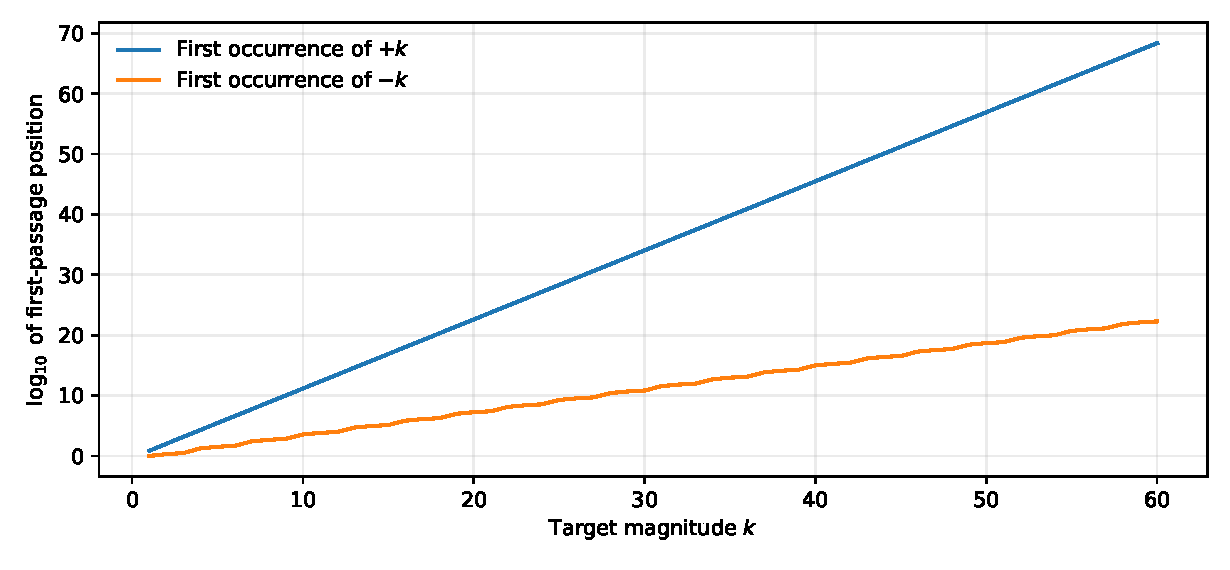
\includegraphics[width=\linewidth]{figures/first_passage_growth.pdf}
\caption{First passages to $+k$ and $-k$ for $1\le k\le60$. The two slopes on a logarithmic scale reflect $\log U_k=k\log\mu+O(1)$ and $\log L_k=(k/3)\log\mu+O(1)$.}
\end{figure}

\subsection{Consequences for enumerated parity sequences}
Let $e(k)$ be the $k$-th positive integer $n$ for which $\lfloor n\sqrt3\rfloor$ is even, and let $o(k)$ enumerate the odd case, both with $k\ge1$. The counts through $N$ are
\[
 E(N)=\frac{N+S(N)}2,\qquad O(N)=\frac{N-S(N)}2.
\]
Hence $e(k)=2k+O(\log k)$ and $o(k)=2k+O(\log k)$. Their exact counting identities are
\[
 e(k)-2k=-S(e(k)),\qquad o(k)-2k=S(o(k)).
\]
In fact, the extreme constants transfer as follows:
\begin{equation}\label{eq:enumerationlimits}
\begin{array}{c|cc}
&\displaystyle\liminf_{k\to\infty}\frac{\cdot-2k}{\log k}
&\displaystyle\limsup_{k\to\infty}\frac{\cdot-2k}{\log k}\\[5pt]\hline
 e(k)&-1/\log\mu&3/\log\mu\\[3pt]
 o(k)&-3/\log\mu&1/\log\mu
\end{array}
\end{equation}
For completeness, the upper positive records $U_h$ themselves are positive steps, and the next step $U_h+1$ is negative because $U_h$ ends a positive run. All $L_h$ for $h\ge4$ end negative runs, so $L_h+1$ is a positive step. The values at these successors are $h-1$ and $1-h$, respectively. These four subsequences attain the four bounds in \eqref{eq:enumerationlimits}; their sequence indices are asymptotic to half their positions, so replacing $\log N$ by $\log k$ changes the denominator only by $O(1)$. This also shows that neither enumerated parity sequence has bounded error from $2k$.

\section{An infinite even-trace family}\label{sec:general}
The proof depends less on the particular number $\sqrt3$ than on a quadratic unit whose trace is even.
Fix an even integer $D\ge4$, and define
\begin{equation}\label{eq:generalconstants}
 \gamma_D=\frac{D+\sqrt{D^2-4}}2,\quad
 \beta_D=\gamma_D^{-1},\quad
 \mu_D=\gamma_D^2.
\end{equation}
The identities $\gamma_D+\beta_D=D$ and $\beta_D^2-D\beta_D+1=0$ will be used repeatedly. The roots are irrational: $D^2-4$ lies strictly between $(D-1)^2$ and $D^2$. Define
\begin{align}
 S_D(N)&=\sum_{n=1}^N(-1)^{\lfloor\gamma_Dn\rfloor},\quad S_D(0)=0,\label{eq:generalwalk}\\
 B_D(n)&=\lfloor\gamma_Dn\rfloor,\quad T_D(n)=\lfloor\beta_Dn\rfloor,\label{eq:generalBT}\\
 F_D(n)&=D B_D(n)-n+2D-1.\label{eq:generalF}
\end{align}
For $D=4$, adding the even integer $2$ to the slope does not change the signs, so $S_4=S$.

\begin{theorem}[Even-trace record theorem]\label{thm:general}
List the records of $S_D$ increasingly as $\Rs_0=0,\Rs_1,\ldots$. Then for $q\ge0$ and $0\le j<D$,
\begin{equation}\label{eq:generalrecords}
 \Rs_{Dq+j}=F_D^q(j),\qquad
 S_D(\Rs_{Dq+j})=
 \begin{cases}q,&j=0,\\-((D-1)q+j),&1\le j<D.\end{cases}
\end{equation}
Every orbit $x_q=F_D^q(s)$ satisfies
\begin{equation}\label{eq:generalscalar}
 x_{q+2}=(D^2-2)x_{q+1}-x_q+2(D-1).
\end{equation}
The running-extreme and pointwise limits are
\begin{align}
 \max_{n\le N}S_D(n)&=\frac{\log N}{\log\mu_D}+O(1),&
 \limsup_{N\to\infty}\frac{S_D(N)}{\log N}&=\frac1{\log\mu_D},\label{eq:generalmax}\\
 \min_{n\le N}S_D(n)&=-\frac{(D-1)\log N}{\log\mu_D}+O(1),&
 \liminf_{N\to\infty}\frac{S_D(N)}{\log N}&=-\frac{D-1}{\log\mu_D}.\label{eq:generalmin}
\end{align}
The constants implicit in $O(1)$ may depend on $D$.
\end{theorem}

\begin{proof}
\textbf{Runs and renormalization.}
Suppress the subscript $D$ temporarily. Since $D$ is even,
$(-1)^{\lfloor\gamma n\rfloor}=-(-1)^{\lfloor\beta n\rfloor}$ for $n\ge1$. The runs end at $B(k)$ and have sign $(-1)^k$. For positive $k$,
\[
 B(k)=Dk-T(k)-1.
\]
The first run has length $D-1$, and subsequent runs have length $D$ or $D-1$. Short later runs occur at $k=B(\ell)+1$. Exactly the signed-length argument of \cref{lem:endpoint}, now with $D$ in place of $4$, gives
\begin{equation}\label{eq:generalendpoint}
 S_D(B(k))=S_D(T(k))+1-D\odd(k).
\end{equation}
Thus a negative endpoint adds $-(D-1)$ to the reduced walk value, and a positive endpoint adds $1$.

\textbf{First passages.}
The bound $0<\beta\le2-\sqrt3<1/2$ gives $T(B(m)+2)=m$ just as in \cref{lem:fiber}. For a first passage to a new positive level, the first eligible even run is $B(m)+2$, where $m$ is the preceding positive first passage. For a negative target $-(h+D-1)$, the first eligible odd run is $B(m)+2$ with $m$ the first passage to $-h$. The parity argument and the exclusion of all earlier runs are identical to the proof of \cref{thm:first}, because \eqref{eq:generalendpoint} gives the exact eligibility inequalities. The initial negative first passages are $1,2,\ldots,D-1$.
It remains to identify the lift $B(B(m)+2)$ and its iteration.

\textbf{Affine identities.}
Write $u=\{\gamma m\}$. From $\gamma^2=D\gamma-1$,
\[
 \gamma B(m)=DB(m)-m+\beta u.
\]
Consequently,
\[
 B(B(m)+2)=DB(m)-m+\lfloor2\gamma+\beta u\rfloor
           =DB(m)-m+2D-1=F_D(m),
\]
since $2\gamma+\beta u=2D-\beta(2-u)$ and $0<\beta(2-u)<1$.
A second application gives
\begin{equation}\label{eq:generalsecond}
 B(F_D(m))=(D^2-1)B(m)-Dm+2D^2-D-2.
\end{equation}
Here is a detailed check of the last constant. Before taking the floor, the nonintegral remainder is
\[
 (2D-1)\gamma+\beta^2u
 =2D^2-D-\bigl((2D-1)\beta-\beta^2u\bigr).
\]
Using $D\beta=1+\beta^2$ and $0\le u<1$,
\[
 1<2+\beta^2-\beta
 <(2D-1)\beta-\beta^2u
 \le2+2\beta^2-\beta<2.
\]
Thus its floor is exactly $2D^2-D-2$, proving \eqref{eq:generalsecond}.

\textbf{Ordering and recurrence.}
The lift is strictly increasing, and $F_D(0)=2D-1>D-1$. Hence its orbits on the seeds $0,1,\ldots,D-1$ interleave strictly, just as in the four-phase case. The first-passage construction exhausts all levels and proves \eqref{eq:generalrecords}.
The affine matrix is
\[
 A_D=\begin{pmatrix}-1&D\\-D&D^2-1\end{pmatrix},\qquad
 b_D=\begin{pmatrix}2D-1\\2D^2-D-2\end{pmatrix}.
\]
Its determinant is $1$ and its trace is $D^2-2$. Applying its characteristic identity as in \eqref{eq:matrix}, the first component of
$A_Db_D-(D^2-3)b_D$ is $2(D-1)$, yielding \eqref{eq:generalscalar}.

\textbf{Growth and sharpness.}
For all $m\ge0$,
\begin{equation}\label{eq:generalbound}
 \mu_Dm+D-1<F_D(m)\le\mu_Dm+2D-1.
\end{equation}
Iteration bounds $F_D^q(s)$ between two positive constant multiples of $\mu_D^q$ for large $q$, uniformly over the finitely many seeds $0\le s<D$. Hence its logarithm is $q\log\mu_D+O(1)$. The exact prefix extrema after record $Dq+j$ are
\[
 \max S_D=q,\qquad \min S_D=-((D-1)q+j).
\]
This proves the running-extreme estimates. The subsequences $\Rs_{Dq}$ and $\Rs_{Dq+D-1}$ attain the two pointwise constants, completing the proof.
\end{proof}

\subsection{The rational generating function for the entire family}
\begin{corollary}\label[corollary]{cor:generalGF}
For the record positions of $S_D$,
\begin{equation}\label{eq:generalGF}
 \boxed{\sum_{n\ge0}\Rs_nz^n=
 \frac{\displaystyle\sum_{j=1}^{D-1}z^j+Dz^D-(D-1)z^{D+1}
       +\displaystyle\sum_{j=D+2}^{2D-1}z^j}
 {(1-z)\bigl(1-(D^2-2)z^D+z^{2D}\bigr)}.}
\end{equation}
\end{corollary}
\begin{proof}
Equation \eqref{eq:generalscalar} implies
$\Rs_{n+2D}=(D^2-2)\Rs_{n+D}-\Rs_n+2(D-1)$ for every $n\ge0$.
The initial block is $\Rs_j=j$ for $0\le j<D$. Because
$\beta_D(D-1)=1+\beta_D^2-\beta_D<1$, one has $B_D(j)=Dj-1$ for $1\le j<D$. Thus
\[
 \Rs_D=2D-1,\qquad
 \Rs_{D+j}=(D^2-1)j+D-1\quad(1\le j<D).
\]
Multiplication of the generating series by $1-(D^2-2)z^D+z^{2D}$ leaves the polynomial
\[
 P_D(z)=\sum_{j=1}^{D-1}jz^j+(2D-1)z^D
       +\sum_{j=1}^{D-1}(j+D-1)z^{D+j}
\]
plus $2(D-1)z^{2D}/(1-z)$. Expanding $(1-z)P_D(z)+2(D-1)z^{2D}$ gives exactly the numerator in \eqref{eq:generalGF}.
\end{proof}

\begin{corollary}[A square-root subfamily]
For every integer $d\ge1$, the walk with slope $\sqrt{4d^2-1}$ has the record formulas of \cref{thm:general} with $D=4d$. Each cycle introduces $4d-1$ new negative levels and one new positive level.
\end{corollary}
\begin{proof}
For $D=4d$, $\gamma_D=2d+\sqrt{4d^2-1}$. The difference in slopes is the even integer $2d$, which leaves every parity unchanged.
\end{proof}
The extension therefore includes the walks with slopes $\sqrt3,\sqrt{15},\sqrt{35},\sqrt{63},\ldots$, as well as other slopes when $D$ is even but not divisible by four.

\section{Exact computation and reproducibility}\label{sec:code}
\subsection{No floating-point floor decisions}
For $a=D/2$, the floor used throughout the implementation is
\begin{equation}\label{eq:integerfloor}
 B_D(n)=an+\isqrt\bigl((a^2-1)n^2\bigr),
\end{equation}
where $\isqrt(x)$ is the greatest integer whose square is at most $x$.
For positive $n$, $T_D(n)=Dn-B_D(n)-1$; for zero, $T_D(0)=0$.
These expressions use only integer arithmetic, even when $n$ has hundreds of digits.

For general $D$, the full shrinking identity is
\begin{equation}\label{eq:generalalgorithm}
 S_D(N)=S_D(m)+1-D\odd(k)-(-1)^k\bigl(B_D(k)-N\bigr),
 \quad k=T_D(N)+1,\quad m=T_D(k).
\end{equation}
The argument $m$ is less than $N/2$. Thus the evaluation uses $O(\log(N+1))$ calls to integer operations and square roots on integers with $O(\log(N+1))$ bits, for fixed $D$. This is a count of arithmetic calls, \emph{not} a claim of logarithmic bit complexity.

The following is the core of the executable algorithm. The complete module adds type checks, validation, record generation, and exact prefix extrema.
\begin{lstlisting}[language=Python]
from math import isqrt

def B(n, D=4):
    a = D // 2
    return a*n + isqrt((a*a - 1)*n*n)

def T(n, D=4):
    return 0 if n == 0 else D*n - B(n, D) - 1

def walk_value(n, D=4):
    answer = 0
    while n:
        k = T(n, D) + 1
        m = T(k, D)
        odd = k % 2
        answer += 1 - D*odd - (1 - 2*odd)*(B(k, D) - n)
        n = m
    return answer
\end{lstlisting}
The constant-coefficient recurrence is preferable for generating many record positions: it avoids all square roots after initialization. To obtain $R_{4q+s}$ directly, initialize $x_0=s$, $x_1=F(s)$ and apply \eqref{eq:scalar} $q-1$ times. The code's \texttt{record} method uses precisely this integer procedure.

\subsection{What was actually checked}
The included script \texttt{code/verify.py} was executed using Python integers and \texttt{math.isqrt}. Its default run checks the following independent and cross-consistency properties.
\begin{center}
\begin{tabular}{p{0.49\linewidth}p{0.40\linewidth}}
\toprule
Check & Executed scope\\
\midrule
Direct summation versus shrinking evaluation; all actual records versus the predicted record list & $D=4$, every $0\le N\le2{,}000{,}000$\\[3pt]
The same dense comparisons for the extension & Each $D=6,8,10,12,14,16,18,20$, every $0\le N\le50{,}000$\\[3pt]
Large exact endpoints, predecessor values, lift and scalar recurrence & First 1001 records for $D=4$; up to 286 decimal digits\\[3pt]
Further large-endpoint consistency checks & First 301 records for each $D=6,10,20$\\[3pt]
Original four-phase recurrence and generating function \eqref{eq:gf} & First 1001 coefficients/terms\\[3pt]
General generating function \eqref{eq:generalGF} & First 301 coefficients for each even $D$ from 4 through 20\\
\bottomrule
\end{tabular}
\end{center}
All checks passed. The dense comparison computes each increment directly, without using the shrinking identity. The large-number checks instead evaluate the proved shrinking recursion at huge endpoints; they do \emph{not} enumerate all earlier integers. Their purpose is implementation and indexing validation. Minimality at arbitrary size is established by \cref{thm:first}, not by these finite computations.

\subsection{Files and commands}
The archive contains this \LaTeX{} source and compiled PDF, an exact-arithmetic module, the verification script and its logs, CSV data, optional plotting code, and a README. No external Python packages are needed for the proof checks; only the optional plots use Matplotlib.
\begin{lstlisting}
python code/verify.py
python code/record_walk.py walk 2000000
python code/record_walk.py record 400
python code/record_walk.py extrema 2000000
python code/record_walk.py record 120 --D 6
latexmk -pdf article.tex
\end{lstlisting}
The full record table contains indices $0$ through $1000$. The walk-prefix table contains every position through $20000$. The generalized table includes 101 records for each tested even parameter.

\section{Scope, provenance, and remaining questions}\label{sec:scope}
\subsection{What this argument settles}
The target is the explicit $\sqrt3$ record recurrence \eqref{eq:conj1}--\eqref{eq:conj4}, in the corrected form displayed by Bruin and Fokkink \cite[p.~7]{BF}. The proof supplies the missing first-passage justification and then derives the four-line system. The rational generating function, closed forms, exact prefix extrema, and even-trace family follow from that construction.

The separate $\sqrt2$ record theorem is already established in earlier work and is explicitly recalled as Theorem~3 of \cite{BF}, with attribution to the work cited there as \cite{FFL}. It is not a new result of this report. Likewise, showing logarithmic discrepancy for one walk is not a solution of the general quadratic-irrational record conjecture.

The source \cite{BF} describes an automaton for the $\sqrt3$ recurrence conditional on that recurrence being correct. Our theorem supplies the arithmetic premise for that construction. We have not independently verified its transition diagram or a Walnut certificate and therefore do not present the diagram as a separately certified artifact.

\subsection{Why the extension has a boundary}
The proof uses both $\gamma+\gamma^{-1}=D$ and the evenness of $D$. The first makes the short-run positions another copy of the same Beatty structure. The second preserves signs in the self-reduction. For odd trace, the parity of the short-run position introduces an additional index-dependent sign. For more general quadratic slopes, the continued-fraction structure may require multiple states rather than the single reduced walk in \eqref{eq:generalendpoint}. These observations explain which parts of the present proof would need replacement; they are not proofs of the general conjecture.

Natural next problems are to determine a comparably explicit first-passage map for odd-trace units, to incorporate rational offsets in the exponent, and to relate such maps systematically to Ostrowski automata. The general automaticity question is formulated as Conjecture~7 of \cite{BF}; no assertion about its resolution in full generality is made here.

\subsection{Priority and verification limitations}
The online source check on September 19, 2026 found the selected recurrence still described as experimentally obtained in the cited paper; it did not establish that no separate proof exists elsewhere. The central mathematical claim of this report is consequently precise: the supplied elementary argument proves the displayed recurrence and its stated generalization. It is not a claim of independently confirmed publication priority. The document has been algebraically and computationally audited, but no external referee or formal proof assistant has certified it.

\appendix
\section{A compact proof certificate for the central case}\label{app:certificate}
A reader checking the central result can focus on the following chain of exact statements. Every step is proved in the body of the article.
\begin{align*}
 B(n)&=\lfloor(2+\sqrt3)n\rfloor,
 &T(n)&=\lfloor(2-\sqrt3)n\rfloor;\\
 S(B(k))&=S(T(k))+1-4(k\bmod2),&&k\ge1;\\
 T(B(m)+2)&=m,&&m\ge0;\\
 U_{h+1}&=B(B(U_h)+2),&&h\ge0;\\
 L_{h+3}&=B(B(L_h)+2),&&h\ge1;\\
 B(B(m)+2)&=4B(m)-m+7,&&m\ge0;\\
 B(4B(m)-m+7)&=15B(m)-4m+26,&&m\ge0;\\
 R_{4q+j}&=F^q(j),&&q\ge0,\ 0\le j\le3;\\
 R_{n+8}&=14R_{n+4}-R_n+6,&&n\ge0.
\end{align*}
The genuinely extremal step is the passage from the endpoint identity to the recurrences for $L_h$ and $U_h$. It depends on the first eligible run number and its parity; skipping that argument would leave the main conjecture unproved.

\section{A source and notation audit}\label{app:audit}
The target was taken from the arXiv version of \cite{BF}, whose public abstract page identifies version~2 as revised on March 28, 2025. Its PDF page~7 was inspected directly for the four-line recurrence and its experimental status. The 2008 source \cite{ARL} is the original attribution supplied there; the corrected displayed system in this report follows \cite{BF}, not an unverified reconstruction of the original typesetting.

The notation is local to this report. In particular, $R_n$ is a record \emph{position}, $S(N)$ is a walk \emph{value}, and $U_h,L_h$ are first passages to specified values. The variable $q$ in $R_{4q+j}$ counts complete record cycles; it is not a continued-fraction denominator. All logarithms in asymptotic statements are natural logarithms. The initial record $0$ is included consistently in the proofs, formulas, CSV files, and software.

\begin{thebibliography}{9}
\bibitem{BF}
Henk Bruin and Robbert Fokkink,
\emph{On the records and zeros of a deterministic random walk},
arXiv:2503.11734, version~2, March 28, 2025.
\url{https://arxiv.org/abs/2503.11734v2}.
The selected $\sqrt3$ recurrence is in Section~2, p.~7; the known $\sqrt2$ record result is Theorem~3. Consulted September 19, 2026.

\bibitem{ARL}
J. Arias de Reyna and J. van de Lune,
\emph{On some oscillating sums},
Uniform Distribution Theory \textbf{3} (2008), no.~1, 35--72.
\url{https://pcwww.liv.ac.uk/~karpenk/JournalUDT/vol03/no1/ReyLu08-1.pdf}.
Original attribution for the conjectural program; the corrected target statement was checked in \cite{BF}.

\bibitem{FFL}
R. Fokkink, W. Fokkink, and J. van de Lune,
\emph{Fast computation of an alternating sum},
Nieuw Archief voor Wiskunde \textbf{12} (1994), 13--18.
Bibliographic and historical attribution as given in \cite{BF}.
\end{thebibliography}
\end{document}
